%%%%%%%%%%%%%%%%%%%%%%% file typeinst.tex %%%%%%%%%%%%%%%%%%%%%%%%%%%%%%
%
% This is the LaTeX source for the instructions to authors using
% the LaTeX document class SVMultln with class option 'lnicst'
% for contributions to the Lecture Notes of the Institute for
% Computer Sciences, Social-Informatics and
% Telecommunications Engineering series.
% www.springer.com/series/XXXX       Springer Heidelberg 2007/08/05
%
% It may be used as a template for your own input - copy it
% to a new file with a new name and use it as the basis for
% your article. It contains a few tweaked sections to demonstrate
% features of the package, though.
%
% If you have not much experiences with Springer LaTeX support,
% you should better use the special demonstration file "lnicst.tex"
% included in the LaTeX package for LNICST as template.
%
%%%%%%%%%%%%%%%%%%%%%%%%%%%%%%%%%%%%%%%%%%%%%%%%%%%%%%%%%%%%%%%%%%%%%%%%

\documentclass[lnicst,sechang,a4paper,svlnicst.clo]{svmultln}
\usepackage{amssymb}
\usepackage[tight,footnotesize]{subfigure}
\setcounter{tocdepth}{3}
\usepackage{graphicx}

\usepackage{url}
%\urldef{\mailsa}\path|{stefan.goeller, alfred.hofmann, peter.strasser, lnicst}@springer.com|
\urldef{\mailsa}\path|{vwu3, rhc}@illinois.edu|
\usepackage[pdfpagelabels,hypertexnames=false,breaklinks=true,bookmarksopen=true,bookmarksopenlevel=2]{hyperref}

\begin{document}

\mainmatter  % start of an individual contribution

% first the title is needed
\title{3D Audio Interface for\\Rich Mobile Web Experiences}

% a short form should be given in case it is too long for the running head
%\titlerunning{Lecture Notes of ICST: Authors' Instructions}

% the name(s) of the author(s) follow(s) next
%
% NB: Chinese authors should write their first names(s) in front of
% their surnames. This ensures that the names appear correctly in
% the running heads and the author index.
%
\author{Victor K.Y. Wu\inst{1}%
\and Roy H. Campbell\inst{2}}  %

\authorrunning{V.K.Y. Wu and R.H. Campbell}

% the affiliations are given next
\institute{Department of Electrical Engineering 
\and 
Department of Computer Science\\
University of Illinois at Urbana-Champaign, USA\\
\mailsa
%\\
%\url{http://www.springer.com/series/7911}
}

%
% NB: a more complex sample for affiliations and the mapping to the
% corresponding authors can be found in the file "lnicst.dem",
% that is contained in the LNICST LaTeX support package.
%

\toctitle{3D Audio Interface for Rich Mobile Web Experiences}
\tocauthor{Victor K.Y. Wu and Roy H. Campbell}
\maketitle


\begin{abstract}
We propose a novel paradigm of consuming rich web content in a mobile setting (which are often eyes-free), through a predominantly 3D audio interface.  Web content, formatted in audio, is streamed via the mobile device's network connection, and placed virtually in a 3D audio space.  The user moves in the virtual space, using a variety of human computer interaction (HCI) means, such as voice input, touching, rotating, and shaking the device, as well as hand and head gesturing.  We provide applications benefitting from this paradigm of rich mobile 3D audio web consumption.  We provide system designs, and a system architecture for mobile 3D audio.  Finally, we implement our ideas in a system prototype using the Apple iOS mobile platform.
%The abstract should summarize the contents of the paper and should
%contain at least 70 and at most 150 words. It should be written using the
%\emph{abstract} environment.
\keywords{3D audio, mobile HCI, mobile web}
\end{abstract}

\section{Introduction}
We propose a novel paradigm of consuming rich digital content in a mobile setting (which are often eyes-free), through a predominantly 3D audio interface.  In this paper, we focus on web content, since it is the most relevant and interesting in a variety of applications.  Other types of digital content, such as GPS signals or personal music collections are still important, and we highlight them as well.  

In a typical scenario, web content, formatted in audio, is streamed via the mobile device's network connection, and placed virtually in a 3D audio space.  The 3D audio space is readily achieved through stereo headphones and head related transfer functions (HRTFs).  That is, the user perceives sound streams coming from different locations in her surrounding 3D volume.  The user moves in the virtual space (thus changing her perceived soundscape), using a variety of human computer interaction (HCI) means, such as voice input, touching, rotating, and shaking the device, as well as hand and head gesturing.  This creates a rich audio mobile web experience where users can consume multiple streams of content \emph{simultaneously}.  

For example, consider a person standing in a crowded subway train carrying an Internet-connected smart phone.  She cannot look at her device, but multiple web services are streaming her email messages, financial news, stock updates, and social network updates in audio format.  She is even talking over a VOIP connection.  These and other sound items are virtually located at various positions in the 3D space, relative to the user, as shown in Fig. \ref{fig:space2}.  Initially, she is close to the email stream (Gmail), and listens to important messages.  The finance stream (Yahoo! Finance) is further away, and is relatively quieter.  Later, this stream announces the user's heavily-invested stock price, grabbing her attention.  She rotates her smart phone (without having to look at it), moving closer virtually to the finance stream, to listen to the stock's news more carefully.  The Skype sound item automatically stays close to the user, moving along with her in the 3D space, allowing the VOIP conversation to continue unhindered.

Our simple example illustrates that 3D mobile audio allows for rich mobile web experiences, which are otherwise not possible in visually based mobile systems characterized by small screen sizes and eyes-free settings.  Our paradigm is also readily applied for the visually impaired.  

The rest of the paper is organized as follows.  In Section \ref{sec:Motivations}, we motivate our paradigm and discuss related work.  In Section \ref{sec:Applications}, we provide applications that benefit greatly from mobile 3D audio.  We provide system designs in Section \ref{sec:System designs}, and a system architecture in Section \ref{sec:System architecture}.  In Section \ref{sec:Implementation}, we provide a system prototype implementing our ideas.  Finally, we conclude and discuss future work in Section \ref{sec:Conclusion}.

\begin{figure}
\begin{center}
\includegraphics[clip=true, viewport=-25 100 600 700, width=3in]{space2.eps}
\end{center}
\caption{Consuming multiple audio web streams in 3D audio space.  The ``head" indicates the user in the virtual audio space.  The gradient shading shows that closer web streams are relatively louder. \label{fig:space2}}
\end{figure}


\section{Motivations and Related Work}
\label{sec:Motivations}
Existing mobile web experiences are still far inferior than those enjoyed in traditional desktop (non-mobile) settings.  This is the primary motivation for mobile 3D audio.  We explain how our ideas address the problems associated with the current mobile web paradigm and provide a rich mobile web experience.  Furthermore, we argue that research in mobile 3D audio advances digital systems aimed at visually impaired users.

\subsection{Rich Mobile Web Experiences from a Truly Pervasive Web}
Existing mobile devices have an inherent design flaw.  They are modeled after desktop computers.  In fact, other than the few and relatively new interfaces such as touch and voice input \cite{web:Eyes-Free Android}, mobile devices are just small versions of desktop computers, each equipped with a smaller screen and often, a smaller keyboard.  This results in a very poor web experience.  Small screen sizes prevent users from consuming content efficiently.  (Large screen sizes on the other hand, reduce the mobility of the device.  We are inherently plagued with this tradeoff.)  Furthermore, mobile scenarios are often eyes-free.  That is, a user who is driving, jogging, or standing in a crowded subway train cannot access the web because she cannot view her device.  (In contrast, she has no problem listening to music or any other audio content in these situations.)  

A \emph{truly pervasive} web should not be constrained by access technologies, such as visually based mobile web interfaces.  Rather, it should be constrained by how many processes a user can cognitively handle concurrently.  Our mobile 3D audio paradigm fulfills this requirement by providing a rich web experience wherever network connectivity is available.  For example, drivers rightfully should not be allowed to send text messages, because the distractions are proven to be dangerous \cite{2009NYT}, \cite{2010NYT}.  However, a long distance driver should be able to safely listen to her emails through an audio interface, using her Internet-connected smart phone.  This is the true pervasive web.  Furthermore, when the user does have the choice to view her mobile device, we argue that innovative 3D audio interfaces are still better, since we can achieve much richer web experiences than that of a small screen.
 
\subsection{Enabling Technologies}
Existing mobile hardware is already very powerful.  (For example, the Qualcomm Snapdragon chipset used in smart phones has a 1 GHz processor \cite{web:Snapdragon}.)  Furthermore, mobile broadband Internet access is quickly being deployed all over the world \cite{web:LTE}.  Many cities are already equipped with 3G connectivity, with 4G already in a few others.  The economics of the mobile industry are also allowing increasingly more users to have Internet-connected devices.  In other words, supporting technologies (and the economics therein) already allow for mobile 3D audio.

\subsection{Enabling Human Factors}
The \emph{cocktail party effect} allows a person to focus on an individual sound source, even in the presence of other sounds \cite{1953Cherry} \cite{1999Bronkhorst}.  In cognitive psychoacoustic terms, this is known as \emph{selective attention}.  \emph{Alternating attention} refers to the ability to switch focus between different sound sources.  \emph{Divided attention} refers to the ability to simultaneously focus on multiple sources.  Research in this area of cognitive listening shows that listeners achieve better divided attention if the sound sources are spatially separated, which is rather intuitive \cite{2004Shinn-Cunningham}, \cite{2006Best}, \cite{2008Ihlefeld}.  

Recent research in HCI has demonstrated these human characteristics in modern mobile scenarios.  In \cite{2003Lumsden}, \cite{2004Marentakis}, \cite{2009Brewster}, sound items are placed in a virtual audio circle around the user's head, and the user selects the items using hand or head gestures.  Once the user selects an item (by a head nod in the corresponding direction for example), that content is streamed to her.  This idea has even been customized to a mobile application that allows a user to interface to her music in an entirely eyes-free manner, by placing selection menus in the 3D space, and using device rotations for input \cite{2009Hipui}.  We propose extending this idea to a larger space, which we call the \emph{movable 3D audio space}.  Many sound items are placed in a large virtual 3D audio space.  The items are constantly streaming audio content.  Instead of selecting a particular item, a user chooses to move (using hand or head gestures, or device movements) to different locations in the virtual space, allowing her to consume multiple sound streams at once.  This is similar to the ``audio minimization" techniques in \cite{2009Vasquez}.

\subsection{Digital Systems for the Visually Impaired}
Computer web browsers targeted for visually impaired users are readily available.  However, they do not innovate very much beyond screen reading \cite{2004Parente}, \cite{2005Yu}, \cite{2008Bigham}.  In this paper, we focus on sighted users and the mobile web.  We argue that technologies initially developed for sighted users in mobile environments (which are often eyes-free) will eventually be applied to visually impaired users.  Developing visually impaired technology is difficult because the small market economics do not justify the engineering design costs.  By developing rich 3D audio mobile web interfaces for the sighted in general, visually impaired users gain the added benefit of easily adaptable (if not just transferrable) technologies to them.

\section{Applications}
\label{sec:Applications}
We provide several categories of applications that our paradigm supports.  Obviously, many of these overlap.  And in a typical situation, a user may be engaged in multiple applications from multiple web services at the same time.  (We discuss this further in Sections \ref{sec:System designs} and \ref{sec:System architecture}.)

\subsection{Media Converters and Players}
Media converters and players take web content, convert them to audio format and play them for the user.  For example, users can listen to music streamed from various content websites, in various formats, including video (by extracting only the audio portion of course).  Other types of content include lectures or presentations and text-based content (e.g. news websites and blogs), which can all be easily converted to audio format.  We envision that a media converter and player installed locally on a user device has a generic way to parse web content and convert it into audio (similar to screen readers for the visually impaired).  However, a web service or web content provider might provide more friendly interfaces to audio web users, allowing them richer experiences.  For example, after a user queries a music streaming website for a song, the website could play short audio preview clips of search results, which is arguably better than just a spoken text description.

\subsection{Productivity}
Productivity programs are often the killer applications that drive a technology to maturity.  We envision that mobile 3D audio is no different.  Obviously, many office applications, such as word processing or spreadsheets do not work well in an audio setting for document creation or editing.  But they can be easily accessed through text-to-speech means.  Organizational productivity applications are very important, since users benefit greatly when they are accessed in eyes-free settings.  These include email or messaging, voice calling, calendar or organizers, and mapping or navigation.  For example, a driver can talk on the phone (when it is safe to do so) with a coworker, and at the same time, check her calendar to set up a meeting by accessing her meeting management tool (by accessing the associated stream in 3D audio space).  She may even check her email conversations (to listen to previous meeting minutes) to set up an agenda for the meeting.  We classify another type of productivity application as informational.  These include web streams such as news, stock prices, and weather reports.  Since they require minimal interactivity, these informational web streams are easily implemented.  In fact, web feed or subscription technologies such as RSS (Really Simple Syndication) and podcasting can be readily incorporated.

\subsection{Location-Based}
With the advent of modern web services, the mobile web and positioning technologies such as GPS are becoming extremely important.  One notable example is overlaying the virtual world onto the physical world.  Many services provide some type of geotagging feature.  Users associate (that is, ``tag") physical locations with virtual locations on the web.  As a result, a plethora of information can possibly be written to and read from the virtual locations by users.  This allows for a variety of existing location-based services to be readily incorporated in our designs.  

For example, consider a mapping application such as Google Maps used on a regular computer, where users pan around a map view to look at user-generated reviews (possibly in different media formats) on nearby restaurants and entertainment.  In a navigation setting inside a vehicle, the experience is significantly compromised.  The screen on the device is typically smaller, making panning difficult.  Many systems provide some point of interest (POI) search functionality.  However, the experience is still worsened, since spatial awareness (e.g. relative distances between locations) is lacking.  As well, the entire system is dangerous to use when driving (an eyes-bound activity).  Conversely, consider a mapping and navigation application using our paradigm.  In addition to POI search, a user can move around virtually in 3D audio space, listening for POIs streaming audio information (and maybe even user-generated content).  This allows for some spatial awareness (e.g. relative distances between POIs) to be recovered, even in an eyes-free setting.  For example, using simple hand or head gestures, a driver can move in 3D audio space corresponding to the vicinity near her real physical location, listening to user-generated reviews on POIs.  This is shown in Fig. \ref{fig:gmap}.

\begin{figure}
\begin{center}
\includegraphics[clip=true, viewport=25 200 600 550, width=3in]{gmap.eps}
\end{center}
\caption{The Google Map is traversed in movable 3D audio space.  The red dots are locations determined by Google after a query for ``coffee". \label{fig:gmap}}
\end{figure}

\section{System Designs}
\label{sec:System designs}
We discuss several system designs in general.  In Section \ref{sec:System architecture}, we provide a system architecture that organizes many of these ideas in a coherent manner.

\subsection{Movable 3D Audio Spaces}
The mobile 3D audio web consumption paradigm is based largely on a virtual 3D audio space in which multiple sound sources are streaming content. In the most general setting, both the user and sound items move in multiple spaces.  For example, a user might switch between a work space and a personal space, and thus come into contact with different services (and possibly even other users who share the same spaces).  An item in a 3D space can be generalized to any entity that has interaction.  An item might be as simple as a YouTube video stream, or as complex as a group of users playing a virtual board game.  Items are movable and their trajectories can depend on each other. 

\subsection{Sound Stream Prioritization}
One design that affects sound item trajectories in 3D space is prioritization of the items themselves.  For example, a user may wish to have access to her email at all times.  Then her email item may be preset to stay with her, even if she moves in the space.  As well, she may not want too many items in her immediate area, distracting her focus.  Other items may thus be dynamically pushed aside as she moves.  For instance, in Fig. \ref{fig:space2}, as the user moves up, her Gmail item moves along with her, and the Facebook item is automatically pushed to the left.

Notifications and alerts are a form of prioritization, and are very natural in an audio setting.  For example, in Fig. \ref{fig:space2}, the Google Talk and Citibank items are far away from the user.  If a message is received through Google Talk, a short notification sound plays close to the user.  She may then choose to ignore it, or move towards the Google Talk item, and start a chat conversation.  Similarly, if Citibank suspects somebody has stolen the user's credit card credentials, it issues an alert sound close to the user.  Since this is critical, all other items may be automatically disabled until the user responds to the alert.

Instead of using sounds, we can use keywords or phrases that a user can hear and process, even if the audio streams producing these are far away in the 3D space.  In particular, studies have shown that a user is able to recognize somebody speaking her name, even if that audio source is out of focus and far away \cite{1959Moray}.  (For example, in Fig. \ref{fig:space2}, the user likely hears her name, even if it is streamed by the Google Reader item far away.)  In our design, we could allow a user to first tag several interest words or phrases.  For example, these may be, ``New York Yankees", ``Yo-Yo Ma", ``Simpsons", and ``Vinton Cerf", representing the user's interests in sports, music, television, and technology.  Whenever one of these words is about to be streamed, the system automatically replaces it with the user's name, capturing her attention, even if the audio stream is far away.  The user then locates the audio stream in virtual space and moves to it.  The audio stream may replay the user's name for several moments, allowing her time to locate it.  (In the meantime, the actual stream may be buffered if it is a real-time stream.)  

In an alternative design, if an audio stream comes across a tagged interest word or phrase, it automatically moves near the user.  The user then focuses in on that stream or pushes it away in virtual space (using some input mechanism).  This alternative design removes the need for a user to locate a stream of potential interest to her.  However, it may create an unpleasant experience if many streams are frequently appearing in her vicinity.   

\subsection{Sound Encoding}
Thus far, we have assumed that sounds themselves are relatively agnostic to the system.  However, in general, we can encode sound according to where the user is in 3D audio space.  We have already assumed that further away sounds should be relatively quieter (by definition of the virtual space mimicking a real-world scenario where sound volume decays over distance).  Therefore, a simple design is to just stop streaming a sound source (saving computing and networking resources) if the user is far away from it.  (In this case, we consider ``muting" as a degenerate form of sound encoding.)

Another observation is that users tend to be able to recover less information from a far away sound item, since the sound is relatively softer, and the user is likely focused on another sound nearby.  If we model this situation as a channel (in the communications theory sense) between the sound source and the user, we see that the channel capacity is reduced as the sound is positioned further away in 3D audio space.  Thus, if we try to push too many ``bits" through this narrow pipe, some of them are inevitably dropped.  Therefore, we should encode the sound with a lower ``information rate", in a psychoacoustic sense.  (We do not define this rigorously.  However, it is the subject of future work with regard to mobile 3D audio.)  Practically, low-rate encoding can be achieved by reducing the speed of sounds.  For example, if a news website sound item is far away, it can stream the text of articles slower than usual by allowing more delay between audio samples.  Alternatively, the sound source may choose instead to stream a summary or a simpler version of its content.  In this case, the news item streams only headlines when it is far away.  As the user moves closer to the news item, the news item begins to stream detailed article text.  As well, the encoding can also be in space, in addition to time.  That is, when the user is far away from the news item, it streams only headlines from various news sections.  As the user moves closer, the item actually splits into multiple sound items, which locate themselves in the vicinity of the original item in virtual space.  Each of the new sound items represents a different news section, and streams its own headlines.  Finally, the user can move close to the one of these new items, causing it to stream detailed news article text.

\begin{figure}
\begin{center}
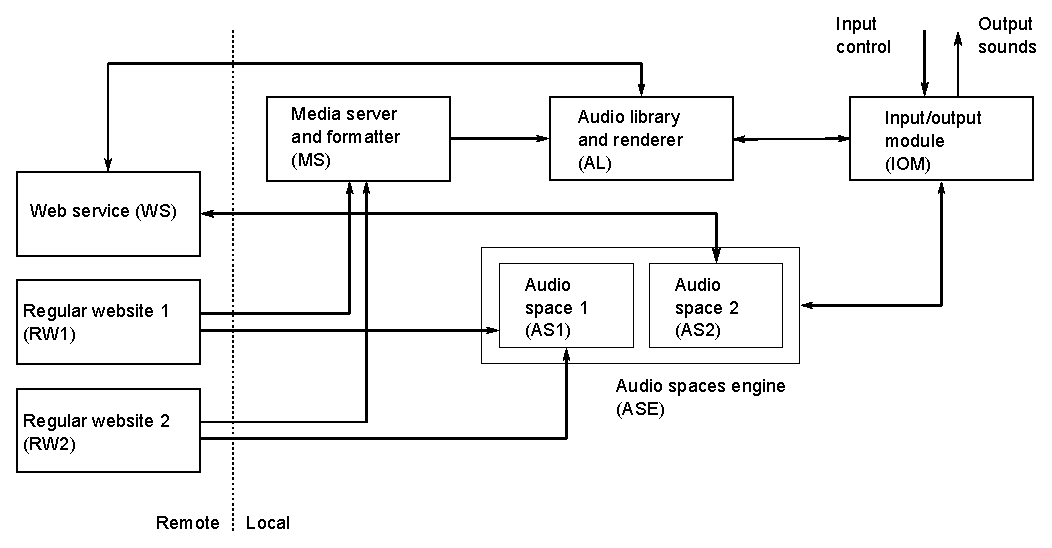
\includegraphics[width=4.5in]{system_architecture.eps}
\end{center}
\caption{Mobile 3D audio system architecture \label{fig:System architecture}}
\end{figure}

\section{System Architecture}
\label{sec:System architecture}

We provide a system architecture in Fig. \ref{fig:System architecture}.  Components to the right of the vertical dashed line are all contained within a mobile device.  Components to the left are remote entities from the web. 

\subsection{Overview}
The audio spaces engine (ASE) maintains all the state information of the various audio streams in all the audio spaces.  This includes the locations of the audio streams in 3D audio spaces, and the user's location.  The input/output module (IOM) is an interface between the user and the underlying system components.  That is, the user gives input control signals such as touch or shake gestures, and voice inputs.  IOM then translates these signals into commands such as moving within and switching between audio spaces.  The commands may be even more interactive, such as leaving an audio comment on a blog post.  The underlying system components update themselves based on these commands and report back to IOM.  IOM then collects the resulting output audio and sends it back to the user.

\subsection{Audio Spaces Engine (ASE)}
ASE contains all the relevant audio information to model how a user perceives a soundscape, given her location.  Note that this component does not contain any audio content.  (Actual audio content is stored in the audio library.)  ASE is composed of distinct audio spaces.  Each audio space encapsulates information such as sound item locations, number of sound items, and user location, if the user is in that particular audio space.  Furthermore, the audio spaces are also interactive.  As we discuss later, a web service may directly control an audio space, moving sound items around, perhaps reacting to user movement or other actions.  Note that each audio space is sandboxed apart from each other in ASE, for a stable and secure design.  

\subsection{Non-optimized Websites}
Consider two cases when a user visits a website.  In the first, the website is a traditional visually based site, unaware of the audio capabilities of the user's device.  In the second, the website is optimized to provide the user a rich audio experience.

In the first case, the mobile device first establishes a connection with the remote server.  This is RW1 in Fig. \ref{fig:System architecture}.  RW1 sends visually formatted content (such as text, audio, or video), which is relayed to the media server (MS) on the device.  MS converts the content to audio and stores it in the audio library (AL).  ASE then organizes the sound locations in an audio space (AS1 in Fig. \ref{fig:System architecture}).  This is done according to local device preferences set by the user, since RW1 has no idea that its content is being formatted into audio.  ASE determines the perceived soundscape of the user.  This information is given to IOM.  IOM uses the soundscape information to ask AL to render and aggregate the sounds accordingly.  The result is returned to IOM, and passed to the user as a single stereo signal.  The perceived soundscape is constantly updated as the user moves in sound space.  If the user visits another website, the parsed content may also be assigned to the same audio space, as shown by RW2 in Fig. \ref{fig:System architecture}.

For example, suppose a user with a mobile device first visits a local news website, represented by RW1 in Fig. \ref{fig:System architecture}.  The website returns a webpage containing three news articles and the local weather, in text format.  The text content is sent to MS where it is converted to audio, and then stored in AL.  In particular, the news articles are stored as three audio files, and all of them are tagged with the same library identifier, $ID_{news}$.  The weather report audio file is tagged with $ID_{weather}$.  This is shown in Table \ref{tab:content1}.  ASE creates two sound items corresponding to the news and weather, and places them in AS1.  Each sound item is characterized by its associated library ID, and its virtual location in 3D audio space.  Thus, AS1 only stores a table of sound items, shown in Table \ref{tab:sound items 1}.  It does not contain any actual audio information.  (Audio files are stored in AL.)  In this case, the two sound items are located at $\left(100,0,0\right), \left(-100, 0, 0\right)$, two preset locations customized by the user.  The movable user location $\left(x,y,z\right)$ is also stored in the table.  (Note the user might even be outside AS1, and in AS2 for example.)  Suppose the user is located closer to the news item.  With a simple audio propagation model, ASE determines that $80\%$ and $30\%$ maximum volume of the news and weather audio files, respectively, should be used as part of the user's perceived soundscape (ultimately her modeled head related transfer function).  This information (along with the respective library IDs, $ID_{news}$ and $ID_{weather}$) are passed to IOM.  IOM requests the actual audio from AL (using the library IDs as keys).  AL thus produces an aggregate stereo audio signal that combines $80\%$ maximum volume of the three news audio files (looped in series) and $30\%$ maximum volume of the weather audio file.  As the user moves in AS1, the volume proportions change, so that AL is constantly re-rendering the aggregate output stereo audio signal.  Suppose later the user visits another website, RW2 in Fig. \ref{fig:System architecture} (without ``leaving" RW1).  RW2 is a finance website with stock quotes and an investment advice program video stream.  Two more sound items are added to AS1, with the corresponding audio files added to AL.  Now, a total of four sound items are in AS1.  So as before, depending on the location of the user in AS1, ASE sends the appropriate information to IOM.  IOM then requests the aggregate stereo audio signal from AL as before, but now with the output signal composed of up to four components.  Note that since stock quotes are updated regularly, and the investment advice program is a video stream, the device has to periodically query RW2 for new content, which eventually updates the audio files in AL.  This situation mimics existing web browsers having multiple tabs open, connecting the user to multiple websites.  The audio content stored in AL and the sound items in AS1 for this case of two simultaneous connections to RW1 and RW2 are shown in Tables \ref{tab:content2} and \ref{tab:sound items 2}.

\begin{table}
\caption{Audio content stored in AL for connection to RW1}
\centering
\begin{tabular}{| c | c |}
\hline
\textbf{Audio Content} & \textbf{Library ID} \\
\hline
News article 1 & $ID_{news}$ \\
News article 2 & $ID_{news}$ \\
News article 3 & $ID_{news}$ \\
Weather report & $ID_{weather}$ \\
\hline
\end{tabular}
\label{tab:content1}
\end{table}

\begin{table}
\caption{Sound items in AS1 for connection to RW1}
\centering
\begin{tabular}{| c | c | c |}
\hline
\textbf{Sound Item (or User)} & \textbf{Library ID} & \textbf{Virtual Location in Audio Space} \\
\hline
News & $ID_{news}$ & $\left(100,0,0\right)$ \\
Weather & $ID_{weather}$ & $\left(-100,0,0\right)$ \\
User & - & $\left(x, y, z\right)$\\
\hline
\end{tabular}
\label{tab:sound items 1}
\end{table}

\begin{table}
\caption{Audio content stored in AL for simultaneous connections to RW1 and RW2}
\centering
\begin{tabular}{| c | c |}
\hline
\textbf{Audio Content} & \textbf{Library ID} \\
\hline
News article 1 & $ID_{news}$ \\
News article 2 & $ID_{news}$ \\
News article 3 & $ID_{news}$ \\
Weather report & $ID_{weather}$ \\
Stock quotes & $ID_{stocks}$ \\
Investment video & $ID_{invest}$\\
\hline
\end{tabular}
\label{tab:content2}
\end{table}

\begin{table}
\caption{Sound items in AS1 for simultaneous connections to RW1 and RW2}
\centering
\begin{tabular}{| c | c | c |}
\hline
\textbf{Sound Item (or User)} & \textbf{Library ID} & \textbf{Virtual Location in Audio Space}\\
\hline
News & $ID_{news}$ & $\left(100,0,0\right)$ \\
Weather & $ID_{weather}$ & $\left(-100,0,0\right)$ \\
Stock quotes & $ID_{stocks}$ & $\left(0, 100, 0\right)$\\
Investment video & $ID_{invest}$ & $\left(0, -100, 0 \right)$\\
User & - & $\left(x, y, z\right)$ \\
\hline
\end{tabular}
\label{tab:sound items 2}
\end{table}

\subsection{Audio-Optimized Websites}
In the second case, when the device connects to an audio-optimized website, a web service replies, asking for additional, device-specific information and resource permissions in order to create an optimized mobile 3D audio web experience.  This may include the web service requesting multiple shared or not shared audio spaces, a limit on the allowed total number of sound items, and the allocated bandwidth for audio streams.  As well, the web service may ask for available and allowable user interfaces.  The device may reply with, for example, a touch screen with a certain resolution, and an accelerometer with certain sensitivity settings.  After providing this initial information, the device assigns the web service direct access to possibly multiple audio spaces.  In Fig. \ref{fig:System architecture}, we show one web service (WS) with direct access to one audio space (AS2).  WS directly sends formatted audio content to AL, bypassing MS, easing the computational load of MS and AL.  With this level of control, web services can provide customizable and rich experiences for users

For example, suppose a user visits a social networking website, represented by WS in Fig. \ref{fig:System architecture}.  After requesting for device information and permissions, the social network has total control of AS2 and is allowed to place up to 10 sound items in it.  It is allowed to store up to 30 audio files in AL, with each file not exceeding 3 MB in size, and 3 minutes in duration.  With these constraints, the social network creates a customized 3D audio space in AS2 for the user.  That is, on the server side, the audio space is represented by a large virtual space consisting of all the user's friends as sound items.  Since WS can only place up to 10 sound items, only a portion of that large virtual space is replicated in AS2, corresponding to the 10 closest friends with respect to the user's current location, in AS2.  This is shown in Fig. \ref{fig:social network}.  As the user moves in AS2, its location is fed back to WS directly.  This is indicated by the arrow pointing from AS2 to WS in Fig. \ref{fig:System architecture}.  Thus, WS can update the sound items in AS2 accordingly in real-time.  (That is, the 10 closest friends change as the user moves.)  WS sends the audio files (of social networking status updates and other social information) corresponding to the 30 closest friends of the user's current location, to AL, and updates them as the user moves.  The larger subset of friends in AL (audio files) than in AS (sound items with no audio information inherently) enables the system to react fast enough, since there is a delay for WS to send audio files to AL, as the user moves quickly in AS2.  WS also modifies the entire structure of friend placement in the audio space, over multiple sessions, depending on which friends the user is near more often.  These friends are placed closer together, and nearer to the user when she visits the social networking website in subsequent visits to the social network.

\begin{figure}
\begin{center}
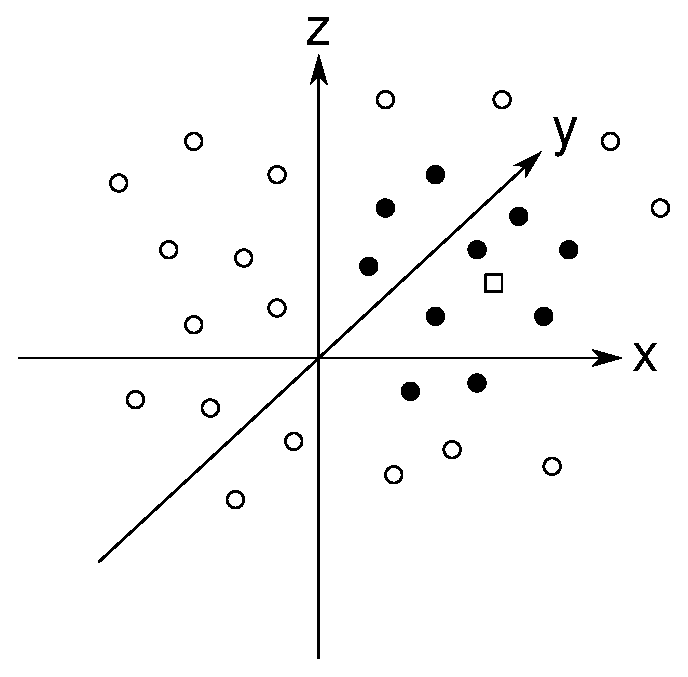
\includegraphics[clip=true, viewport=0 0 350 350, width=4in]{social_network.eps}
\end{center}
\caption{3D audio space representation of a social network.  The user is represented by the square.  The circles are the user's friends.  They are all placed in 3D audio space.  The filled circles indicate the 10 closest friends.  The locations of the user and of these 10 friends are stored in AS2.
\label{fig:social network}}
\end{figure}

\section{Implementation}
\label{sec:Implementation}

\begin{figure}
\centering
    \subfigure[3D audio navigation screen]{\includegraphics[width=2.3in]{iPhone01.eps}} 
    \subfigure[Content selection screen]{\includegraphics[width=2.3in]{iPhone02.eps} } 
\caption{System prototype on the Apple iOS mobile platform \label{fig:iPhone}}
\end{figure}

We integrate many of these ideas in a system prototype.  We design and program a mobile application on the Apple iOS mobile operating system platform.  It is currently available on the Apple App Store \cite{2010iPhone app}.  The application is an audio RSS reader.  It retrieves RSS feeds, converts them to audio, and plays them in 3D audio space.  The user moves in the space with touch gestures and shaking the device.

\subsection{Prototype Design and Functionality}
The application is composed of two screens, as shown in Fig. \ref{fig:iPhone}.  The first is the navigation screen, where the user moves in 3D audio space.  The second is the content selection screen, where the user can select up to six RSS feeds (and locally stored music files).  If the user is in the first screen, a simple two-finger tap anywhere brings up the second screen.  A back button labelled ``3D" on the second screen returns the user to the first screen.

The application downloads up to six RSS feeds and converts them to audio files.  (A feed is re-downloaded and re-converted after a user selects it on the second screen if it is more than 15 minutes old.)  The audio files are placed in fixed positions in 3D audio space and played (in a looping manner).  The six positions are $\{$north, south, east, west, up, down$\}$, equidistant from the origin.  In the first screen, the user controls her movement in audio space.  Touch dragging forward or backward and left or right on the screen moves her x-y coordinates.  Tapping the top half of the screen moves her up on the z-axis, and tapping the bottom half moves her down.  Shaking the device returns her to the origin.  

The navigation interface is entirely eyes-free.  The user senses her location by listening to how relatively loud the audio feeds are, and how the soundscape changes as she moves (a feedback mechanism).  (The screen does display the user's current coordinates nonetheless.)  This prototype demonstrates a rich mobile RSS experience.  The user can pre-select her desired content, and listen to them in an eyes-free situation.  Switching between feeds is extremely simple.  The user can even listen to feeds simultaneously, as well as listen to ``background" music.

\subsection{Audio Implementation Details}
In our prototype, the downloaded RSS feed content is in text format.  Therefore, we convert the text to audio using a text-to-speech (TTS) engine.  This is part of MS in Fig. \ref{fig:System architecture}.  We have one audio space in ASE.  The dragging, tapping, and shaking gestures are passed from IOM into the audio space, which calculates the position of the user.  Based on the user location, AL renders the audio files, and aggregates them into a single stereo sound.  This is accomplished with OpenAL, a cross-platform API for simulating 3D audio \cite{OpenAL}.  Basically, we pass in the relative audio locations and user location (and orientation) in 3D space, and the API returns the perceived stereo sound.  This is constantly updated as the user moves in the 3D audio space.

\section{Conclusion and Future Work}
\label{sec:Conclusion}
In this paper, we propose a new paradigm of 3D audio mobile web consumption.  This allows the user a rich digital experience, even on a small device with a small screen.  We motivate our paradigm and provide applications.  We provide system designs and a system architecture.  Finally, we implement many of our ideas in a system prototype on the Apple iOS mobile platform.

Future work includes further developing our system designs.  There are still many interactive audio web interfaces that we have yet to explore.  These include designing standardized audio sounds to help the user navigate in the 3D audio spaces.  As well, we predominantly discuss the spatial aspect of sound in this paper.  This is inherently related to a sound's volume.  We wish to explore other aspects such as pitch (frequency), quality (the harmonics of a tone), and reverberation (echoes).  We also plan to exploit the temporal aspect of sound, in addition to spatial.

We plan to incorporate more components in our system architecture (Fig. \ref{fig:System architecture}) in a more complete implementation.  This includes both integrating a more general audio spaces system on the local device side, as well as developing audio-aware web services on the remote side.  In particular, there needs to be many additional web protocols that cater to 3D audio information flow.  This will allow web services to provide personalized audio web experiences in a standardized manner.

We also plan to do extensive user studies to test our designs.  In particular, we want to know how the cocktail party effect depends on the vastly different types of content on the web.  For example, background music likely requires very little attention.  But we want to characterize the differences in attention required for listening to emails versus listening to social network streams, for example.

\subsubsection*{Acknowledgments.} 
We acknowledge many people who contributed at various stages to this work.  Dr. Virginia Way Tong Chu was heavily involved early on in conceptualizing movable 3D audio spaces, as being analogous to the real physical world.  Professor Alex Kirlik, an expert in audio perception, provided a lot of context to the human side of the problem.  Professor Yih-Chun Hu helped frame the problems and issues from an engineering design standpoint.  And Mirko Montanari provided valuable feedback on the structure and flow of the manuscript.

%\begin{thebibliography}{4}

%\bibitem{jour} Smith, T.F., Waterman, M.S.: Identification of Common Molecular
%Subsequences. J. Mol. Biol. 147, 195--197 (1981)

%\bibitem{lnicstchap} May, P., Ehrlich, H.C., Steinke, T.: ZIB Structure Prediction Pipeline:
%Composing a Complex Biological Workflow through Web Services. In: Nagel,
%W.E., Walter, W.V., Lehner, W. (eds.) Euro-Par 2006. LNCS, vol. 4128,
%pp. 1148--1158. Springer, Heidelberg (2006)

%\bibitem{book} Foster, I., Kesselman, C.: The Grid: Blueprint for a New Computing
%Infrastructure. Morgan Kaufmann, San Francisco (1999)

%\bibitem{proceeding1} Czajkowski, K., Fitzgerald, S., Foster, I., Kesselman, C.: Grid
%Information Services for Distributed Resource Sharing. In: 10th IEEE
%International Symposium on High Performance Distributed Computing, pp.
%181--184. IEEE Press, New York (2001)

%\bibitem{proceeding2} Foster, I., Kesselman, C., Nick, J., Tuecke, S.: The Physiology of the
%Grid: an Open Grid Services Architecture for Distributed Systems
%Integration. Technical report, Global Grid Forum (2002)

%\bibitem{url} National Center for Biotechnology Information, http://www.ncbi.nlm.nih.gov

%\end{thebibliography}

\begin{thebibliography}{99}

\bibitem{web:Eyes-Free Android}
Announcing Eyes-Free Shell For Android, (Apr. 2009), http://google-opensource.blogspot.com/2009/04/announcing-eyes-free-shell-for-android.html

\bibitem{2009NYT} Parker-Pope, T.: What Clown on a Unicycle? Studying Cellphone Distraction. New York Times, (Oct. 2009), http://well.blogs.nytimes.com/2009/10/22/what-clown-on-a-unicycle-studying-cell-phone-distraction/

\bibitem{2010NYT} Richtel, M.: Forget Gum. Walking and Using Phone Is Risky. New York Times, (Jan. 2010), http://www.nytimes.com/2010/01/17/technology/17distracted.html

\bibitem{web:Snapdragon}
The Snapdragon Platform. Qualcomm, \\http://www.qualcomm.com/products\_services/chipsets/snapdragon.html

\bibitem{web:LTE}
Evolution to LTE report. Global Mobile Suppliers Association, (Apr. 2010), http://www.gsacom.com/news/gsa\_298.php4

\bibitem{1953Cherry} 
Cherry, E.C.: Some Experiments on the Recognition of Speech, with One and with Two Ears. Journal of the Acoustical Society of America, vol. 25, no. 5, pp. 975-979 (Sep. 1953)

\bibitem{1999Bronkhorst} 
Bronkhorst, A.W.: The Cocktail Party Phenomenon:  A Review of Research on Speech Intelligibility in Multiple-Talker Conditions. Acta Acustica united with Acustica, vol. 86, pp. 117-128 (Jan. 2000)

\bibitem{2004Shinn-Cunningham} 
Shinn-Cunningham, B.G., Ihlefeld A.: Selective and Divided Attention:  Extracting Information from Simultaneous Sound Sources. In: International Conference on Auditory Display (ICAD), Sydney, Australia (Jul. 2004)

\bibitem{2006Best} 
Best, V., Gallun, F.J., Ihlefeld, A., Shinn-Cunningham, B.G.: The Influence of Spatial Separation on Divided Listening. Journal of the Acoustical Society of America, vol. 120, no. 3, pp. 1506-1516 (Sep. 2006)

\bibitem{2008Ihlefeld} Ihlefeld, A., Shinn-Cunningham, B.G.: Spatial Release from Energetic and Informational Masking in a Divided Speech Identi�cation Task. Journal of the Acoustical Society of America, vol. 123, no. 6, pp. 4380-4392 (Jun. 2008)

\bibitem{2003Lumsden} Lumsden, J., Brewster, S.: A Paradigm Shift:  Alternative Interaction Techniques for Use with Mobile and Wearable Devices. In: Conference of the Centre for Advanced Studies on Collaborative Research (CASCON), Toronto, Canada, pp. 197-210 (Oct. 2003)

\bibitem{2004Marentakis} Marentakis, G., Brewster, S.: A Study on Gestural Interaction with a 3D Audio Display. In: International Conference on Human Computer Interaction with Mobile Devices and Services (Mobile HCI), Glasgow, United Kingdom (Sep. 2004) Lecture Notes in Computer Science (LCNS), vol. 3160, pp. 180-191 (2004)

\bibitem{2009Brewster} Brewster S., Murray-Smith, R., Crossan, A., Vasquez-Alvarez, Y., Rico, J.: The GAIME project: Gestural and Auditory Interactions for Mobile Environments. In: Whole Body Interaction Workshop, ACM Conference on Human Factors in Computing Systems (CHI), Boston, MA (Apr. 2009)

\bibitem{2009Hipui} Hipui Funkyplayer, http://www.hipui.com/funkyplayer/

\bibitem{2009Vasquez} Vasquez-Alvarez, Y., Brewster, S.: Audio Minimization: Applying 3D Audio Techniques to Multi-Stream Audio Interfaces. In: Poster Session International Workshop on Haptic and Audio Design (HAID), Dresden, Germany (Sep. 2009)

\bibitem{2004Parente} Parente, P.: Audio Enriched Links: Web Page Previews for Blind Users. In: International ACM SIGACCESS Conference on Computers and Accessibility (ASSETS), Atlanta, GA, pp. 2-8 (Oct. 2004)

\bibitem{2005Yu} Yu, W., Kuber, R., Murphy, E., Strain, P., McAllister, G.: A Novel Multimodal Interface for Improving Visually Impaired People�s Web Accessibility. Virtual Reality, vol. 9, no. 2, pp. 133-148 (Mar. 2006)

\bibitem{2008Bigham} Bigham, J., Prince, C., Ladner, R.: WebAnywhere: A Screen Reader On-the-Go. In: ACM International Cross-disciplinary Conference on Web Accessibility (W4A), Beijing, China, pp. 73-82 (Apr. 2008)

\bibitem{1959Moray} Moray, N: Attention in Dichotic Listening: Affective Cues and the Influence of Instructions. The Quarterly Journal of Experimental Psychology, vol. 11, pp. 56-60 (Feb. 1959)

\bibitem{2010iPhone app} Wu, V.K.Y.: 3D Audio RSS/Music Player. Apple App Store, http://itunes.apple.com/us/app/3d-audio-rss-music-player/id363753578?mt=8

\bibitem{OpenAL} OpenAL, http://connect.creativelabs.com/openal/

\end{thebibliography}

\end{document}
